\documentclass{lecture}

\title{Neuro-symbolic integration}
\subtitle{Automated planning}
\author{Jedrzej Potoniec}

\graphicspath{{03_planning}}


\usepackage{algorithm}
\usepackage[noend]{algorithmic}

\let\vec\bm

\def\vx{{\bm{x}}}
\def\vz{{\bm{z}}}

\newcommand{\function}[1]{\textsc{#1}}

\newcommand{\init}{{\vx^{I}}}
\newcommand{\goal}{{\vx^{G}}}
\newcommand{\zinit}{{\vz^{I}}}
\newcommand{\zgoal}{{\vz^{G}}}
\newcommand{\encode}{\function{encode}}
\newcommand{\decode}{\function{decode}}

\newcommand{\Xtr}{\mathcal{X}}
\newcommand{\Ztr}{\mathcal{Z}}
\newcommand{\xtr}[1][\defaultindex]{\vx^{#1}}
\newcommand{\ztr}[1][\defaultindex]{\vz^{#1}}

\begin{document}

\frame{\titlepage}

\begin{frame}{Bibliography}
    The lecture is based on:
    \begin{itemize}
        \item Masataro Asai, Hiroshi Kajino, Alex Fukunaga, Christian Muise:
        Classical Planning in Deep Latent Space. J. Artif. Intell. Res. 74: 1599-1686 (2022)
        \item Masataro Asai, Hiroshi Kajino, Alex Fukunaga, Christian Muise:
        Symbolic Reasoning in Latent Space: Classical Planning as an Example. Neuro-Symbolic Artificial Intelligence 2021: 52-77        
    \end{itemize}
    
    The software is available at \url{https://github.com/guicho271828/latplan}
\end{frame}

\begin{frame}{Propositional planning (STRIPS)}
    \begin{itemize}
        \item a set of boolean variables $V$
        \item an initial state $\subseteq V$
        \item a goal condition $\subseteq V \cup \lnot V$
        \item a set of actions:
        \begin{itemize}
            \item precondition $\function{pre}(a) \subseteq V \cup \lnot V$
            \item add effect $\function{add}(a) \subseteq V$
            \item delete effect $\function{del}(a) \subseteq V$
        \end{itemize}
        \pause
        \item An applicable action: $\function{pre}(a)$ is satisfied
        \item Applying an action: $s'=s\backslash \function{del}(a) \cup \function{add}(a)$
        \item The task: to find a sequence of actions $a_1, \ldots, a_n$ such that:
        \begin{itemize}
            \item $s_0$ is the initial state
            \item $s_{i}=a_n(s_{i-1})$
            \item the goal is satisfied in $s_n$
        \end{itemize}
        \pause
        \item Typically FOL, but even propositional generalizes
    \end{itemize}
\end{frame}


\begin{frame}{Example}
    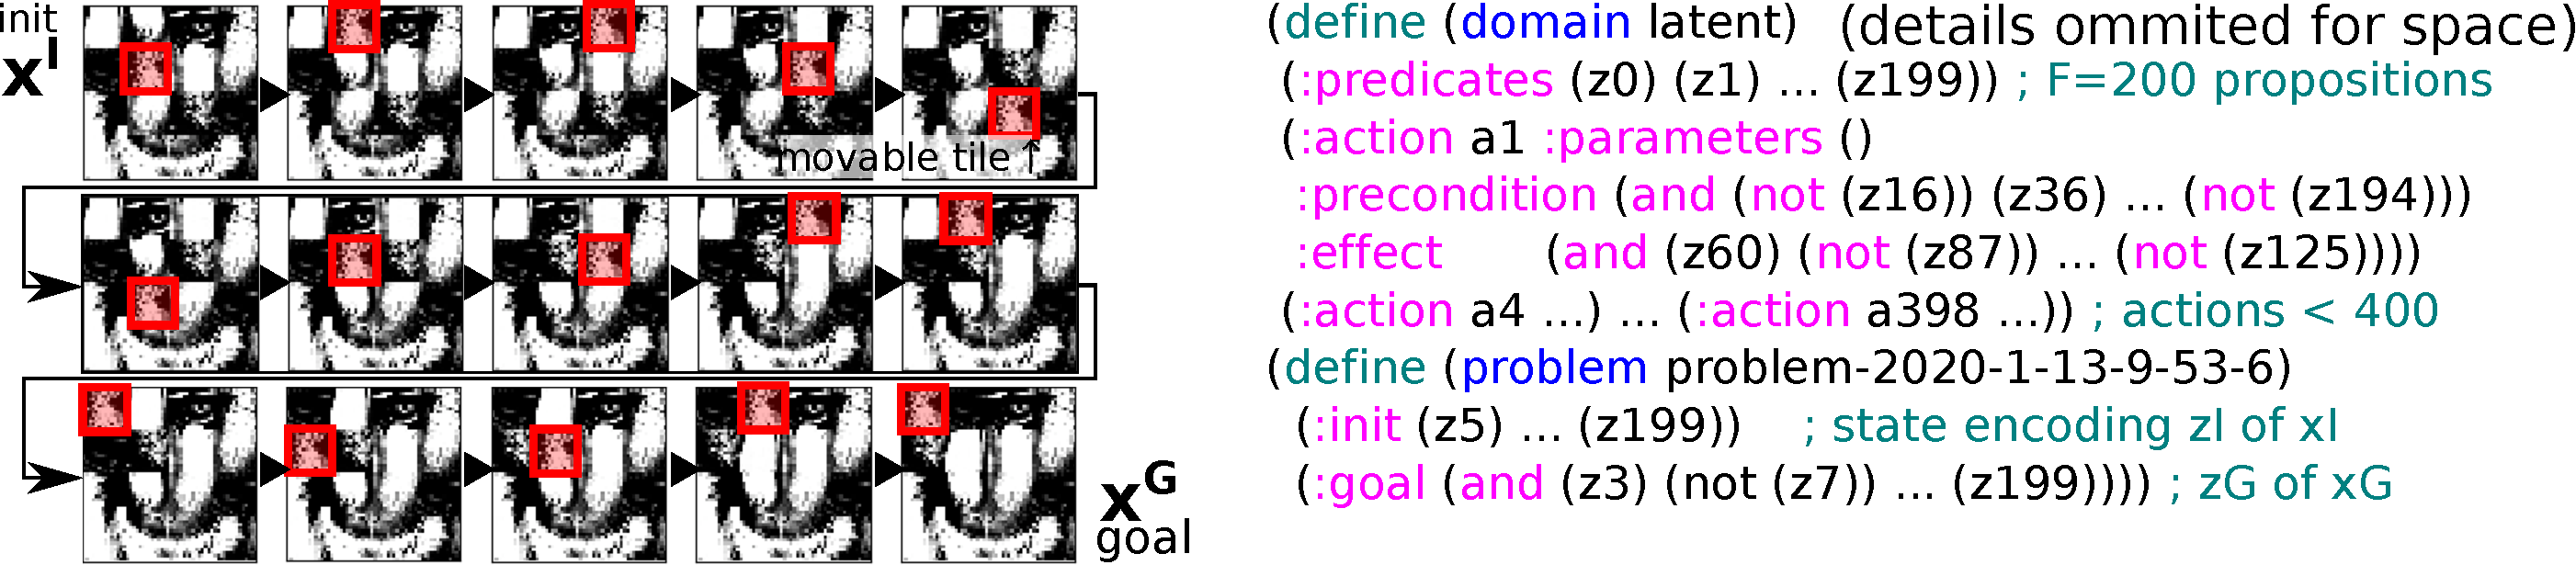
\includegraphics[width=\textwidth]{img___15puzzle-with-pddl.pdf}
\end{frame}

\begin{frame}{Problems with classical planning}
    \begin{itemize}
        \item knowledge acquisition bottleneck
        \item new, unforeseen situations
        %\item symbol grounding problem
    \end{itemize}            
\end{frame}

\begin{frame}{General problem formulation}
    \begin{block}{}
    We consider the problem of robustly, automatically map between such
subsymbolic representations and the formal specifications required by symbolic systems.
    \end{block}
\end{frame}

\begin{frame}{Goal}
    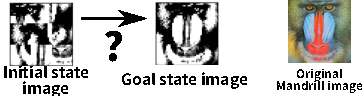
\includegraphics[width=\textwidth]{img___mandrill-intro-new.pdf}    
    \pause
    \begin{itemize}
        \item  a domain-independent system
        \item  unlabeled images showing the valid moves
        \item finds an optimal solution
        \item  has no prior assumptions/knowledge (e.g., “sliding objects”, “tile arrangement”)
        \item must acquire all knowledge from the images
    \end{itemize}
\end{frame}

\begin{frame}{Good think I don't research automated planning}
    
\includegraphics[width=\textwidth]{phd112006s.png}
    \source{\url{https://phdcomics.com/comics/archive/phd112006s.gif}}
\end{frame}

\begin{frame}{Latplan}
    \begin{itemize}
        \item deep discrete generative model
        \item trained on a set of subsymbolic inputs (not necessarily images)
        \item unsupervised training
        \item maps a problem to a symbolic planning instance, invokes a planner, visualizes the plan
    \end{itemize}   
\end{frame}


\begin{frame}{Symbol grounding}
    \begin{itemize}
        \item an unsupervised process of establishing a mapping from
        noisy, continuous and/or unstructured inputs to a set of discrete, identifiable entities;
        \item in general PDDL: objects, predicates, propositions, actions, problems, and domains
        \item a separate problem: symbol generation
    \end{itemize}
\end{frame}

\begin{frame}{Action Model Acquisition}
    \begin{block}{}
    An Action Model is a symbolic data structure representing the causality
in the transitions of the world. 
    \end{block}
\end{frame}

\begin{frame}[fragile]{Training Phase}        
        \begin{algorithmic}[1]
         \REQUIRE Dataset $\Xtr$, untrained machine learning model $M$
         \STATE Trained model $M' \gets \function{train}(M,\Xtr)$ \label{line:train}
         \STATE $M'$ provides functions $\encode$ and $\decode$. \label{line:provide-encode-decode}
         \STATE PDDL domain file $D \gets \function{generateDomain}(M')$ \label{line:generate-domain}
         \RETURN $M', D$
        \end{algorithmic}
        \vfill
        $\Xtr=\{x^{i,0}, x^{i,1}\}_i$
        \begin{itemize}
            \item $x^{i,0}$ before an action
            \item $x^{i,1}$ after the action
        \end{itemize}
        \vfill
\end{frame}

\begin{frame}[fragile]{Planning Phase}        
       \begin{algorithmic}[1]
         \REQUIRE $M', D$, initial state observation $\init$, goal state observation $\goal$
         \STATE Encode $\init, \goal$ into propositional states $\zinit, \zgoal$ \label{line:encode-init-goal}
         \STATE PDDL problem file $P \gets \function{generateProblem}(\zinit, \zgoal)$ \label{line:generate-problem}
         \STATE Plan $\pi=(a_0, a_1, \ldots, ) \gets \function{solve}(P, D)$ using a planner (e.g., Fast Downward) \label{line:plan}
         \STATE State trace $(\zinit=\vz^0,\  \vz^1=a_0(\vz^0),\  \vz^2=a_1(\vz^1),\  \ldots, \zgoal) \gets \function{simulate}(\pi, \zinit, D)$
        using a plan validator for PDDL, e.g., VAL.  \label{line:simulate}
         \RETURN Decode an observation trace $(\init=\vx^0, \vx^1, \vx^2, \ldots, \goal)$. \label{line:decode-plan}
        \end{algorithmic}        
\end{frame}

\begin{frame}{Propositional Symbol Grounding with State AutoEncoder}
    \begin{itemize}
        \item can generalize: unseen world states $\to$ known symbols
        \item noise-resistant: similar images $\to$ same representation
        \item decodable: symbols $\to$ images
    \end{itemize}
\end{frame}

\begin{frame}{State AutoEncoder with Binary-Concrete VAE}
    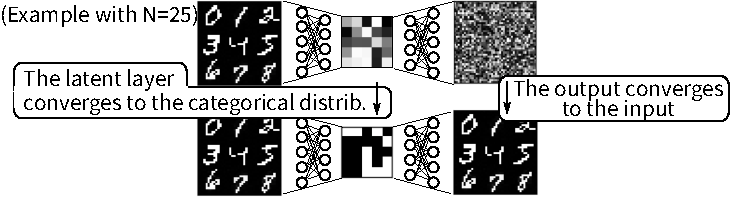
\includegraphics[width=\textwidth]{img___train-state-ae.pdf}
    \pause
    \begin{gather*}
        \text{reconstruction loss} + \text{KL divergence} \\
        z = BC_\tau(l) = \sigma\left(\frac{l+\function{Logistic}(0, 1)}{\tau}\right) \\
        \lim_{\tau\to0} BC_\tau(l) = \begin{cases} 0 & l<0 \\ 1 & l\geq 0 \end{cases}
    \end{gather*}
    $\tau$ is a function of the training epoch, e.g., an exponential schedule
\end{frame}

\begin{frame}{BC VAE $\to$ propositional symbols}
    \begin{itemize}
        \item each dimension = propositional variable
        \item number of dimensions = a hyperparameter
    \end{itemize}
\end{frame}

\begin{frame}{Action Symbol Grounding with Action AutoEncoder}
    \begin{enumerate}
        \item Identify actions (e.g., \emph{slide-up-8-at-position-1-2} -- but no labels)
        \item Identify preconditions and effects
        \item Translate to PDDL
    \end{enumerate}
\end{frame}

\begin{frame}{Major components}
    \begin{itemize}
        \item $\function{ACTION}(\text{pre-state}, \text{post-state}) = \text{action id}$ 
        \item $\function{APPLY}(\text{action id}, \text{pre-state}) = \text{post-state}$
        \item $\function{APPLICABLE}(\text{pre-state}) = \text{action id}$
    \end{itemize}
\end{frame}

\begin{frame}{Complete architecture}
    \vfill
    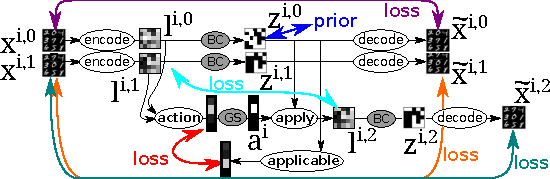
\includegraphics[width=\textwidth]{img___latplan___ama3.pdf}
    \pause
    \vfill
    3 reconstruction losses + 3 KL divergences
    \vfill
\end{frame}

\begin{frame}{The Symbol Stability Problem}
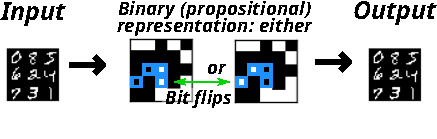
\includegraphics[width=\textwidth]{img___zsae___unstable.pdf}\\
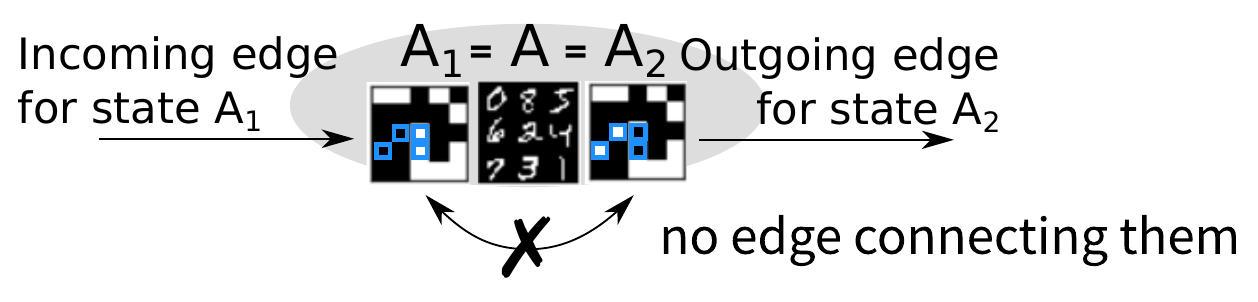
\includegraphics[width=\textwidth]{no_edge.png}
\end{frame}

\begin{frame}{A stable symbol}
    \begin{block}{}
        A symbol is \emph{stable} when its referents are identical for the same environment, under some equivalence relation (e.g., invariance or noise threshold on the observation).
    \end{block}
\end{frame}

\begin{frame}{Stabilizing symbols}
    \vfill
    \begin{itemize}
        \item<+-> in the planning phase, dispense with randomness altogether
        \item<+-> in the training phase, replace $B(0.5)$ with $B(\varepsilon)$      
    \end{itemize}
    \vfill
    \includegraphics<+->[width=\textwidth]{img___zsae___overview.pdf}
    \vfill
\end{frame}

\begin{frame}{Action Symbol Grounding with Action AutoEncoder}
    \begin{enumerate}
        \item[\cmark] Identify actions
        \item[\cmark] Identify preconditions and effects
        \item[\xmark] Translate to PDDL
    \end{enumerate}
    \pause
    $\function{Apply}(\text{action id}, \text{pre-state})$ is an arbitrary neural network, not necessarily concisely translatable to \[\text{pre-state}\backslash \function{del}(\text{action id}) \cup \function{add}(\text{action id})\]
    \pause
    \alert{Non-conformance to the syntactical restrictions in the
    target formal language}
\end{frame}

\begin{frame}{Cube-Space AutoEncoder}
    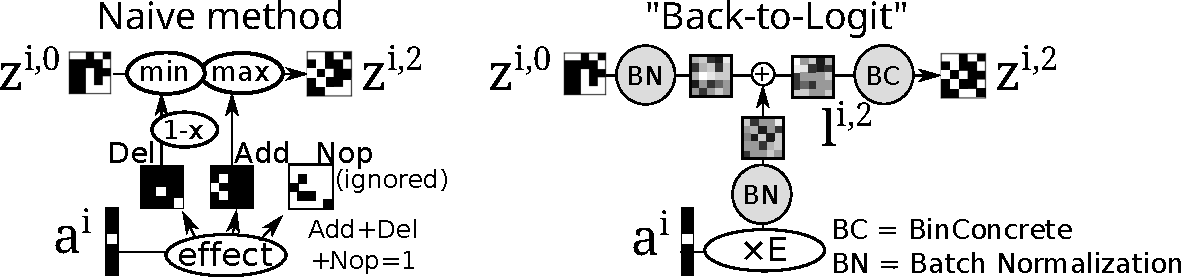
\includegraphics[width=\textwidth,clip=true,trim=0 0 350 0]{img___latplan___cube-space.pdf}
    \only<2->{\alert{$z^{i,2}$ cannot be used in the KL divergence}}
\end{frame}

\begin{frame}{Cube-Space AutoEncoder}
    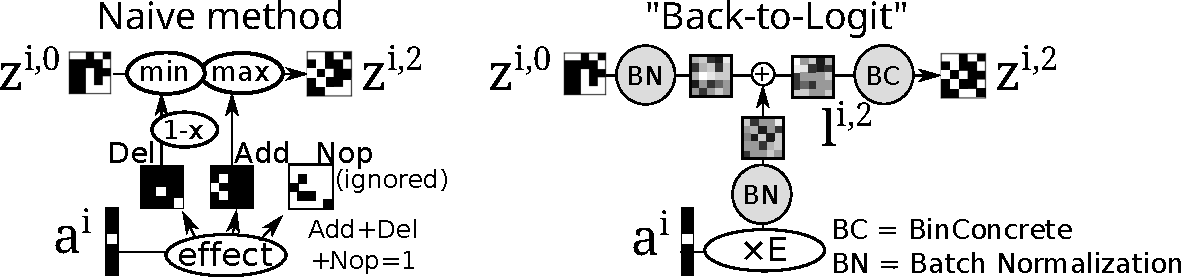
\includegraphics[width=\textwidth,clip=true,trim=220 0 0 0]{img___latplan___cube-space.pdf}
    \vfill
    \pause
    \begin{align*}
        z^{i,2} = BC_\tau(\function{apply}(z^{i,0}, a^i)) = & BC_\tau(m(z^{i,0}) + \function{effect}(a^i)) \\        
        = & BC_\tau(BN(z^{i,0}) + BN(Ea^i)) \\
    \end{align*}
    \vfill
\end{frame}

\begin{frame}{PDDL extraction}
    \begin{align*}
        \function{add}(a) = & \function{apply}(a, 0) \\
        \function{del}(a) = & 1-\function{apply}(a, 1) \\
    \end{align*}    
    \pause
    \begin{align*}        
        Z^0(a) = & \{z^0 | \exists z^1\, \function{action}(z^0, z^1)=a \} \\
        \function{pre}(a) = & \{f | \forall z^0\in Z^0(a)\, z_f^0=1\} \cup \{\lnot f |\forall z^0\in Z^0(a)\, z_f^0=0\} \\        
    \end{align*}
    \pause
    \alert{This is a rough heuristics!}
\end{frame}

\begin{frame}{Bidirectional Cube-Space AE (BiCSAE)}
    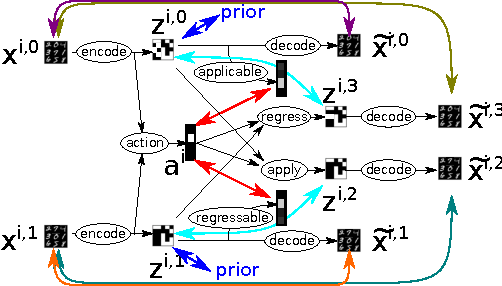
\includegraphics[width=\textwidth]{img___latplan___ama4.pdf}
    \alert{We will skip it to maintain a shred of sanity}
\end{frame}

\begin{frame}{Experimental domains: MNIST 8-Puzzle}
    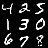
\includegraphics[width=.45\textwidth]{img___static___vanilla___mnist___init.png}
    \hfill
    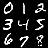
\includegraphics[width=.45\textwidth]{img___static___vanilla___mnist___goal.png}\\
    \vfill
    $42\times 42$ pixels, $9!$ states, $\approx 10^6$ transitions
    \vfill
\end{frame}

\begin{frame}{Experimental domains: Scrambled Photograph 15-puzzle}
    
\includegraphics[width=.45\textwidth]{img___static___vanilla___mandrill___init.png}
    \hfill
    
\includegraphics[width=.45\textwidth]{img___static___vanilla___mandrill___goal.png}\\
    \vfill
    $56\times 56$ pixels, $16!$ states
    \vfill
\end{frame}

\begin{frame}{Experimental domains: LightsOut}
    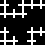
\includegraphics[width=.45\textwidth]{img___static___vanilla___digital___init.png}
    \hfill
    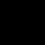
\includegraphics[width=.45\textwidth]{img___static___vanilla___digital___goal.png}\\
    \vfill
    $45\times 45$ pixels, $n=5$, $2^{n^2}$ states, $n^2\cdot 2^{n^2}$ transitions
    \vfill
\end{frame}

\begin{frame}{Experimental domains: Twisted LightsOut}
    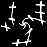
\includegraphics[width=.45\textwidth]{img___static___vanilla___twisted___init.png}
    \hfill
    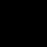
\includegraphics[width=.45\textwidth]{img___static___vanilla___twisted___goal.png}\\
    \vfill
    $45\times 45$ pixels, $n=5$, $2^{n^2}$ states, $n^2\cdot 2^{n^2}$ transitions
    \vfill
\end{frame}

\begin{frame}{Experimental domains: Photo-realistic Blocksworld}
    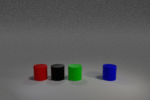
\includegraphics[width=.45\textwidth]{img___static___vanilla___blocks___init-highres.png}
    \hfill
    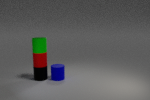
\includegraphics[width=.45\textwidth]{img___static___vanilla___blocks___goal-highres.png}\\
    \vfill
    $30\times 45$ pixels, $4$ objects, $5$ towers, $\approx \infty$ images per state
    \vfill
\end{frame}

\begin{frame}{Experimental domains: Sokoban}
    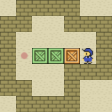
\includegraphics[width=.45\textwidth]{img___static___vanilla___sokoban___sokoban_init_2_False.png}
    \hfill
    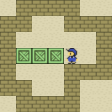
\includegraphics[width=.45\textwidth]{img___static___vanilla___sokoban___sokoban_goal_2_False.png}\\
    \vfill
    $28\times 28$ pixels, $23363$ reachable states, branching factor $1..4$
    \vfill
\end{frame}

\begin{frame}{Experimental setup}
    \begin{itemize}    
        \item 20 random instances solvable in 7 steps (optimal may be shorter)
        \item 20 random instances solvable in 14 steps (optimal may be shorter)
        \item Fast Downward planner: A* with 3 different heuristics + LAMA
        \item resources: 10 min, 8 GB RAM
        \item domain-specific validators
    \end{itemize}
\end{frame}

\begin{frame}{Results (subset, for BiCSAE)}
    \centering
    \begin{tabular}{|r|ccc|ccc|}
        \hline
         & \multicolumn{ 3}{c|}{Blind} & \multicolumn{ 3}{c|}{M\&S} \\
         \hline
 & \textbf{found} & \textbf{valid} & {\textbf{optimal}} & {\textbf{found}} & {\textbf{valid}} & {\textbf{optimal}} \\
        \hline
        Blocks & {33} & {32} & - & {34} & {33} & - \\
        LightsOut & 40 & 40 & {40} & 40 & 40 & {40} \\
        Twisted & 40 & 40 & {40} & 40 & 40 & {40} \\
        Mandrill & 25 & 23 & {23} & \textbf{40} & \textbf{32} & \textbf{32} \\
        MNIST & {40} & 39 & {6} & {40} & 39 & {6} \\        
        Sokoban & {40} & {39} & {38} & {40} & {39} & {38} \\
        \hline
        \end{tabular}
\end{frame}

\begin{frame}{Valid suboptimal plan}
    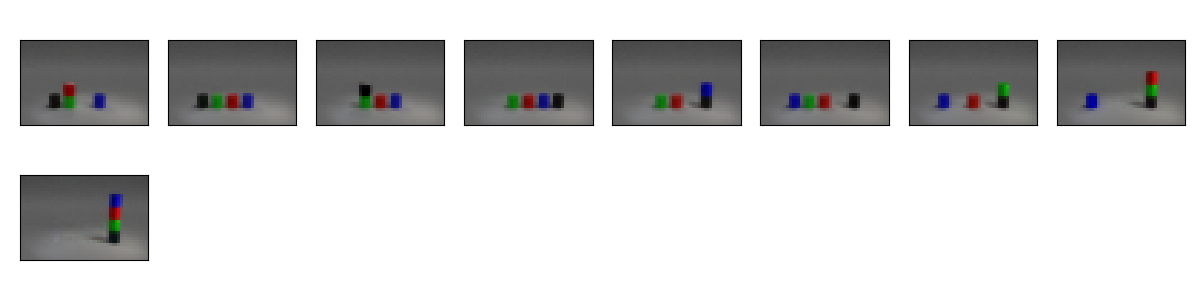
\includegraphics[width=\textwidth]{img___static___examples___014-020-ama3_samples_blocks_cylinders-4-flat_20000_None_None_CubeSpaceAE_AMA4Conv_nozsae2_logs_05-16T00-57-30-000_domain_lmcut_problem_False-1.png}
    \vfill
    The suboptimality is from the PDDL formulation, not from the symbolic planner.
    \vfill
\end{frame}

\begin{frame}{Invalid plan}
    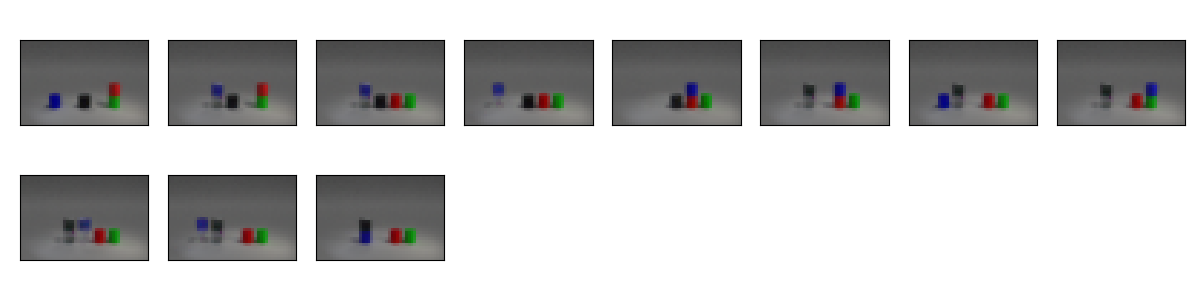
\includegraphics[width=\textwidth]{img___static___examples___007-001-ama3_samples_blocks_cylinders-4-flat_20000_None_None_CubeSpaceAE_AMA4Conv_kltune2_logs_05-06T11-21-56-235_domain_lama_problem_False-1.png}
    \vfill
    Floating blocks
    \vfill
\end{frame}

\begin{frame}{Optimal plan}
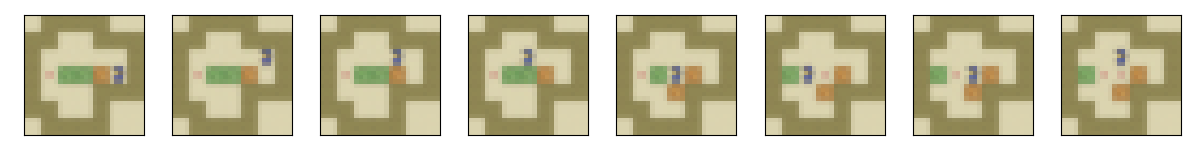
\includegraphics[width=\textwidth]{img___static___examples___007-000-_AMA3Conv_kltune2_logs_05-09T16-42-28-299_domain_blind_problem_False-1.png}
\end{frame}

\begin{frame}{Invalid plan}
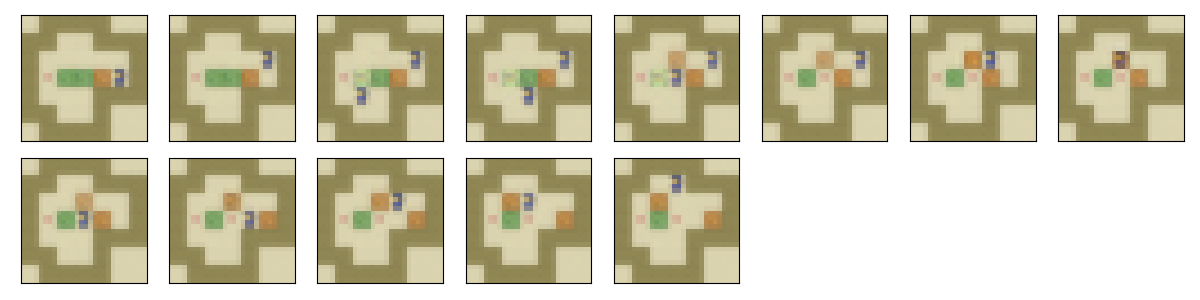
\includegraphics[width=\textwidth]{img___static___examples___014-019-_AMA4Conv_nozsae2_logs_05-15T21-58-49-878_domain_mands_problem_False-1.png} 
\end{frame}

\begin{frame}{Take-home messages}
    \begin{itemize}
        \item Planning heuristics are not tied to the human way of thinking
        \item Latplan is a domain-independent, image-based classical planner
        \item Symbol stability problem
        \item High accuracy $\not\to$ working system
        \item non-conformance to the syntactical restrictions in the target formal language
    \end{itemize}
\end{frame}

\end{document}
